% This is LLNCS.DEM the demonstration file of
% the LaTeX macro package from Springer-Verlag
% for Lecture Notes in Computer Science,
% version 2.4 for LaTeX2e as of 16. April 2010
%
\documentclass{llncs}
%
\usepackage{makeidx}  % allows for indexgeneration
\usepackage{graphicx}
\usepackage[spanish]{babel}
\usepackage{amsmath}
\usepackage{cite}
\usepackage{url}
\usepackage[utf8]{inputenc}

\setcounter{tocdepth}{2}
%
\begin{document}
\frontmatter
\pagestyle{headings}  % switches on printing of running heads

\addtocmark[2]{Sistemas de Recuperación de Información\\ Trabajo Final}
\mainmatter              % start of the contributions
%
\title{Sistemas de Recuperación de Información\\ Trabajo Final}
%
\titlerunning{Sistemas de Recuperación de Información\\ Trabajo Final}  % abbreviated title (for running head)
%                                     also used for the TOC unless
%                                     \toctitle is used
%
\author{Jorge J. Morgado Vega\inst{1} \and Roberto García Rodrígez\inst{1}}
%
% \authorrunning{Ivar Ekeland et al.} % abbreviated author list (for running head)
%
%%%% list of authors for the TOC (use if author list has to be modified)
\tocauthor{Jorge J. Morgado Vega y Roberto García Rodrígez}
%
\institute{Universidad de la Habana, La Habana, Cuba}

\maketitle              % typeset the title of the contribution

\renewcommand\abstractname{Resúmen.}
\renewcommand\keywordname{{\bf Palabras Claves:}}
\begin{abstract}
	La recuperación de información ha sido desde sus inicios una de las tareas
	más arduas en el campo de las ciencias de la computación. Específicamente,
	la recuperación de texto es uno de los subcampos más analizados de esta área.
	El siguiente proyecto propone un sistema de recuperación de texto basado
	en modelos vectoriales. Ofrece, además un sistema de evaluación de los mismos
	sobre varias colecciones reconocidas, así como dos aplicaciones que facilitan
	la interacción del usuario con el sistema.
\keywords{recuperación de información, recuperación de texto, modelos vectoriales}
\end{abstract}
\renewcommand\abstractname{Abstract.}
\renewcommand\keywordname{{\bf Keywords:}}
\begin{abstract}
	Information retrieval has been one of the most arduous tasks in the field
	of computer science since its inception. Specifically, text retrieval is
	one of the most analyzed subfields in this area. The following project
	proposes a text retrieval system based on vector models. It also offers an
	evaluation system of the same on various recognized collections, as well as
	two applications that facilitate user interaction with the system.
\keywords{information retrieval, text retrieval, vector models}
\end{abstract}
%

\tableofcontents
\clearpage

El papel de la investigación en el desarrollo de la ciencia, más que evidente,
es su esencia misma. Naturalmente, la \emph{Recuperación de Información} (RI)
no es una excepción, y su desarrollo progresivo como disciplina ha venido
marcada, para lo bueno y para lo malo, por los resultados de la investigación
realizada.

La RI es un campo donde se realiza una actividad importante de práctica
profesional y, también, de investigación científica. Por un lado, dio lugar a
la aparición de la industria de la información, con sus bases de datos y
sistemas de información, con un marcado componente práctico y profesional
centrado en el uso de las bases de datos para satisfacer las necesidades de
información de los usuarios. Por otro lado, la investigación científica ha
estado dirigida hacia el diseño de \emph{Sistemas de Recuperación de
Información} (SRI) más eficaces, dando lugar a diversas teorías, modelos y
experimentos en los que la evaluación ha ocupado un papel central. A lo largo
de la historia no ha existido una relación muy estrecha entre ambos
componentes, científico y profesional, al menos hasta los últimos años en los
que parece haberse producido un cierto acercamiento y una implementación de
las teorías y modelos experimentales en las aplicaciones comerciales.

La investigación en RI ha favorecido sobre todo la estimulación de ideas; estas
ideas, conforme se han ido explorando y comprobando en sistemas experimentales,
se han convertido en teorías o modelos. Por lo tanto, estas ideas, teorías y
modelos desarrollados han estado influenciados en gran parte por la comprensión
y el conocimiento empírico obtenido a partir de experimentos en los que la
evaluación ha estado omnipresente.

Son muchos los experimentos, tests e investigaciones llevadas a cabo en el
campo de la RI, y también muchas las críticas y discusiones sobre los
resultados obtenidos, derivadas, en su mayoría, por las diferentes
metodologías utilizadas, en parte debidas a la gran variedad de problemas
investigados y, en parte, debidas también a la diversa procedencia académica
de los investigadores.

Concretamente en los SRI se han hecho grandes avances y se ha extendido su uso
de tal forma que nadie se imagina un día despertar y ver que grandes sistemas
de búsqueda en INTERNET, como Google, no existen. Las necesidades crecientes
de la humanidad y la complejización que experimentan los problemas con el paso
del tiempo, fuerzan a la mejora de los modelos e implementaciones con el fin
de tener herramientas cada vez mejores. Se destacan en esta cuestión los
modelos básicos de los SRI: \emph{Modelo Booleano, Vectorial y Probabilístico},
siendo los principales, los cuales sentaron las bases de sistemas más robustos
desarrollados en la actualidad.

En el siguiente trabajo se abordará todo lo referente a las cuestiones más
importantes de un SRI, en este caso utilizando un \emph{Modelo Vectorial},
explicado su diseño, modelado, implementación, procesos por los que transita,
evaluación, ventajas y desventajas.


\newpage

\section{Diseño e Implementación}\label{sec:design}

Para analizar el diseño de la aplicación se realizará una descripción de forma
\emph{top-down}. Primero se mostrarán las capas superiores comenzando por la
interacción del usuario con la aplicación y luego se analizará de forma
detallada el diseño e implementación de cada una de las componentes que
conforman la misma.

De forma general el usuario tiene dos formas de interactuar con la aplicación:
mediante una interfaz de lineas de comando en una terminal (\emph{Command Line
Interface}, CLI por sus siglas en inglés) desarrollada usando \emph{typer} o
mediante una interfaz gráfica desarrollada usando \emph{streamlit}.

Para hacer uso de la aplicación y comenzar a realizar consultas a una base de
datos, el usuario debe realizar primero dos acciones:

\begin{enumerate}
	\item Construir la base de datos.
	\item Construir el modelo de RI de la base de datos construida.
\end{enumerate}

\subsection{Construcción de la base de datos}\label{sec:build-database}

\subsection{Construcción del modelo}\label{sec:model}



\section{Evaluación}\label{sec:eval}

Como parte fundamental de la creación de un SRI se tiene el proceso de
evaluación, donde se determinará la eficacia del mismo.

Para la evaluación del modelo propuesto se cuenta, como procedimiento estándar,
con varias colecciones de pruebas, las cuales contienen lo siguiente:

\begin{enumerate}
    \item Una colección de documentos.
    \item Un conjunto de pruebas a realizar sobre la colección, llamadas
    consultas (\emph{queries}).
    \item Un conjunto de juicios de relevancia, una evaluación mayormente
    binaria sobre la relevancia de las consultas sobre los documentos (en
    algunas de las colecciones utilizadas el espectro de evaluación no es tan
    binario) 
\end{enumerate}

Sobre la estructura de las colecciones utilizadas y descritas con anterioridad,
trabaja el modelo, se realizan comparaciones y cálaculo de métricas que
caracterizan la efectividad del mismo.

\subsection{Métricas empleadas}\label{sec:metrics}

Para realizar un análisis de la efectividad de cada modelo se emplearon 
dversas métricas. Primero, se define como:

\begin{itemize}
	\item RR: Documentos relevantes recuperados.
	\item RI: Documentos irelevantes recuperados.
	\item NR: Documentos relevantes no recuperados.
	\item NI: Documentos irelevantes no recuperados.
	\item P: Precisión.
	\item R: Recobrado.
\end{itemize}

Luego, las métricas usadas son:

\begin{itemize}
\item Precisión:
    $$P = \dfrac{|RR|}{|RR \cup RI|}$$
    Denota la proporción de los documentos relevantes recuperados sobre
	el total de documentos recuperados.\\
\item Recobrado (Recall):
    $$R = \dfrac{|RR|}{|RR \cup NR|}$$
	Denota la proporción de los documentos relevantes recuperados sobre
	el total de documentos relevantes.\\
\item Medida $F_1$:
    $$F_1 = \dfrac{2PR}{P+R} = \dfrac{2}{\frac{1}{P} + \frac{1}{R}}$$
    Medida que armoniza entre Precisión y Recobrado.\\
\item Fallout:
	$$Fallout = \dfrac{|RI|}{|RI\cup NI|}$$
     Denota la cantidad de documentos irrelevantes recuperados sobre el total de
	 documentos irrelevantes.
\end{itemize}

\subsection{Proceso de evaluación}\label{sec:evaluation}

Para describir el proceso de evaluación primero es necesario definir el concepto
de \emph{tope}. Este concepto se define como: los primeros $k$ documentos
resultantes de una consulta.

En el análisis de un modelo se calculan las métricas antes mencionadas, por
cada consulta, para diferentes topes. De estas métricas se extraen valores
estadísticos relevantes como: la media, la desviación estándar, el máximo y
el mínimo, por cada uno de los topes establecido ($2, 4, 6, ..., 50$). Se
analiza además, el comportamiento del promedio de las relevancias.

De esta forma para cada modelo se puede analizar el comportamiento de las métricas
estudiadas a medida que aumentamos la cantidad de documentos recuperados. En las
figuras \ref{fig:cran-eval} y \ref{fig:med-eval} se muestran los resultados
para el modelo de Cran y el modelo de Medline respectivamente. Como se puede
observar, el modelo de Medline, presenta una mayor efectividad.

Se puede apreciar en ambos resultados como el la precisión va disminuyendo y 
el recobrado va aumentando a medida que aumentan la cantidad de documentos
recuperados.

Es notable además que ambos modelos presentan un comportamiento similar con
respecto al promedio de relevancia obtenido en cada tope. Esto muestra que
este valor por si solo no es una métrica útil. No obstante, es interesante
analizar su comportamiento en función de la cantidad de documentos recuperados.

\begin{figure}[htb]%
	\begin{center}
		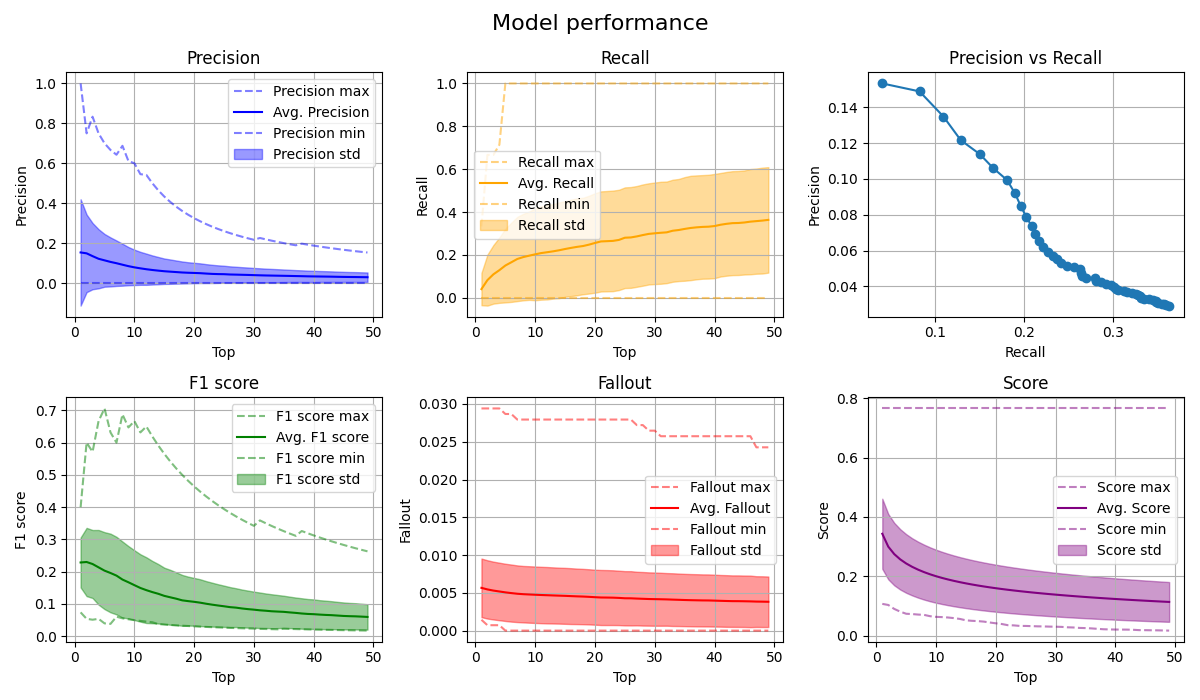
\includegraphics[width=1.0\textwidth]{./cran_eval.png}
	\end{center}
	\caption{Evaluación del modelo de la base de datos \emph{cran}}
	\label{fig:cran-eval}
\end{figure}


\begin{figure}[htb]%
	\begin{center}
		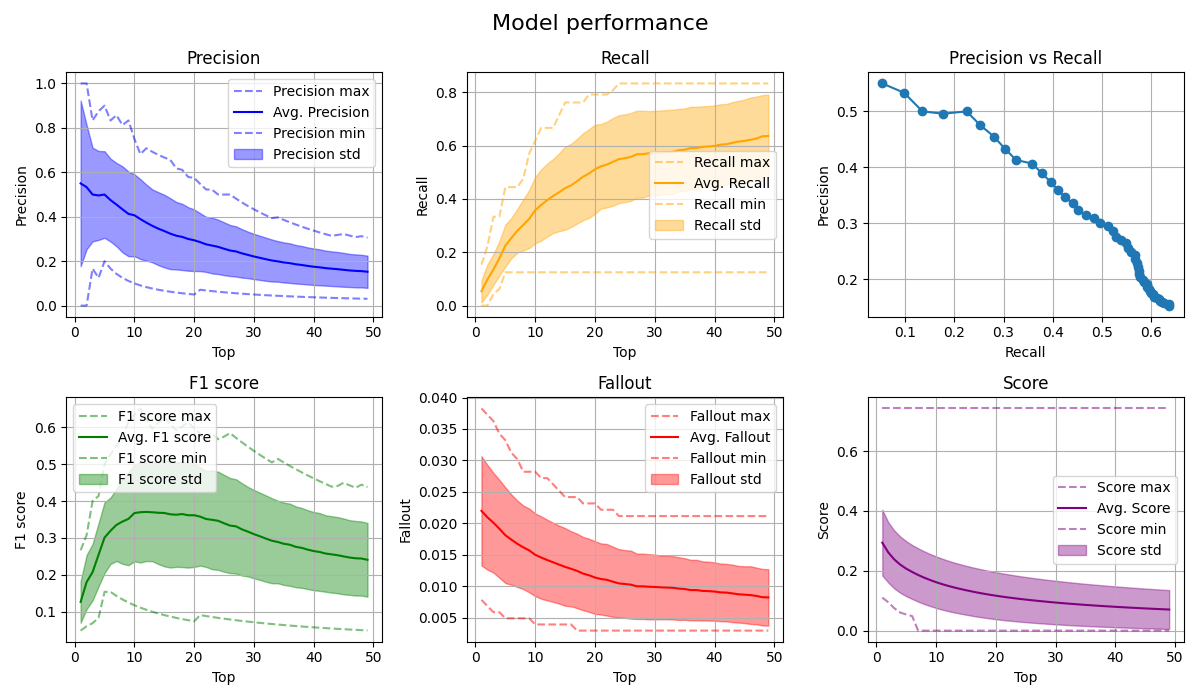
\includegraphics[width=1.0\textwidth]{./med_eval.png}
	\end{center}
	\caption{Evaluación del modelo de la base de datos \emph{med}}
	\label{fig:med-eval}
\end{figure}

Además de la evaluación de un modelo determinando, la aplicación desarrollada
permite mostrar una comparación entre modelos creados con diferentes
parámetros para una misma base de datos. En la figura \ref{fig:cran-comp} se muestra
la comparación entre dos modelos de la base de datos de \emph{cran}. Uno de ellos
(líneas discontinuas) fue construído con una tokenización simple (split), sin
lemtizar, sin stemming, sin quitar las palabras comunes. El otro, por otra parte,
fue construído con utilizando el método de tokenización de \emph{nltk}, con
stemming, lematización, quitando las palabras comunes.

\begin{figure}[htb]%
	\begin{center}
		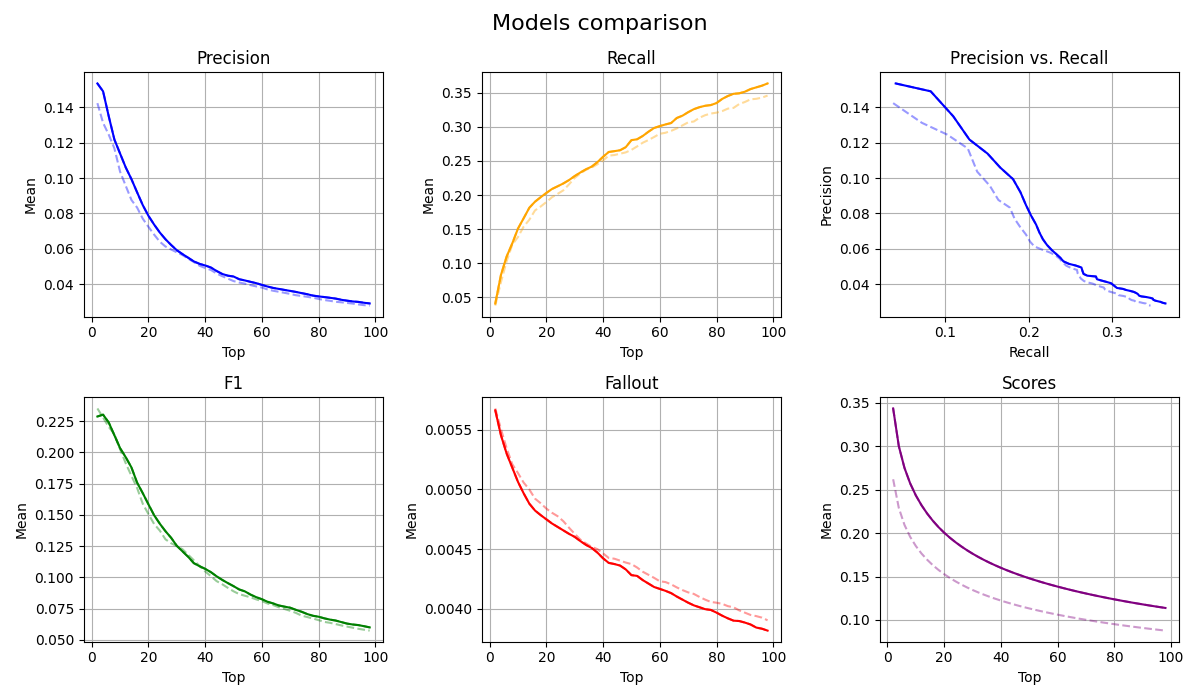
\includegraphics[width=1.0\textwidth]{./cran_comp.png}
	\end{center}
	\caption{Comparación de diferentes modelos para la base de datos \emph{cran}}
	\label{fig:cran-comp}
\end{figure}

Como se puede apreciar, con el nuevo modelo se obtuvo una pequeña mejora en la
precisión y el recobrado. Se muestra también cómo el promedio de fallos disminuyó.


\section{Ventajas y Desventajas}

Como se ha podido apreciar en el desarrollo de este trabajo, \emph{TF-IDF} es
un eficiente y simple algoritmo para hacer coincidir palabras en una consulta
con documentos que son relevantes para esa consulta. Como cada
modelo de RI, este tiene aspectos que lo hacen beneficioso, y al mismo tiempo,
a pesar de la fuerza del modelo, se escapan algunos puntos que le imponen
limitaciones.\cite{ramos, aparicio, mishra}

\subsection{Ventajas}

\subsubsection{Esquema de Ponderación}

El modelo vectorial es muy versátil y eficiente a la hora de generar
\emph{rankings} de precisión en colecciones de gran tamaño, lo que le hace
idóneo para determinar la equiparación parcial de los documentos. De esta
forma, aunque se recuperen \emph{n} documentos relevantes a una consulta, la
misma relevancia viene dada por una métrica de \emph{ranking} y tendremos, de
cierta manera, ''relevancia dentro de la relevancia''

\subsubsection{Coincidencia Parcial}

La estrategia de coincidencia parcial permite la recuperación de documentos
que se aproximen a los requerimientos de la consulta. De esta forma quizas se
tengan documentos recuperados que no cumplan con todas las características de
la consulta, sino una parte considerable de la misma, los cuales son relevantes
a la consulta hecha.

\subsubsection{Medida de Similitud}

Se demuestra la eficacia de la \emph{fórmula del coseno} como métrica que
ordena los documentos de acuerdo al grado de similitud con la consulta,
aprovechádose de resultados \emph{geométrico-algebráicos} que plantean la
similitud entre vectores de acuerdo al coseno del ángulo que ellos determinan. 

\subsection{Desventajas}

\subsubsection{Estructura del Lenguaje}

Al ser un modelo estadístico-matemático, no tiene en cuenta la estructura
sintáctico-semántica del lenguaje natural. En general recupera documentos
cuando hay igualdad de palabras entre el documento y la consulta no tiene en
cuenta, por ejemplo, sinónimos.

\subsubsection{Umbral de Relevancia}

Establecer un umbral para definir que documentos son relevantes y cuales no es
un valor que no es fijo y fiable a cada colección, o sea, para cada colección
hay que probar y reajustar para ver que umbral se ajusta mejor y permite tener
métricas de evaluación más compensadas.

\subsubsection{Independencia de términos}

El modelo asume la independencia mutua entre los términos indexados, cuando,
como suele suceder en la actualidad, muchas veces existe una correlación
evidente entre los propios términos. Por ejemplo, es muy probable que en
textos científicos las palabras \emph{sujeto} y \emph{espécimen} aparezcan
altamente relacionadas.


\newpage

\section{Conclusiones}\label{sec:conc}

En el trabajo presentado se mostraron las características de un SRI utilizando
una implementación de un \emph{Modelo Vectorial (tf-idf)}. Se explica su
diseño, siendo este, uno de las esquemas más usados en la actualidad. Se
detallan las distintas etapas del proceso desde la realización de una consulta,
y como esta es procesada, hasta la recuperación de los documentos relevantes a
la propia consulta. Se explican los algoritmos utilizados en la creación del
modelo así como el uso de varias colecciones de prueba para su evaluación.
Se debatieron, además, de forma ctítica, los principales beneficios y
limitantes que existen en el uso de estos sistemas, los cuales permiten
analizar posibles mejoras a realizar en futuras investigaciones.

La implementación del SRI mostrado dio resultados positivos, la sencillez del
modelo hace que su eficacia pruebe la fortaleza de este algoritmo. Se
evidencia la efectividad del modelo en la colecciones usadas, lo cual se
demuestra en las métricas usadas en la evaluación. Sin duda alguna en
el mundo cambiante de la RI se necesitaran de algoritmos más potentes y otras
mejoras en estos modelos para estar a la altura de la creciente era de la
información.


\newpage

Como propuestas a modo de recomendación sobre el trabajo se pueden señalar
varios aspectos interesantes como: el uso e incorporación de retroalimentación
al modelo con la cual se ganaría en rendimiento y precisión del mismo; la
implementación de algoritmos de \emph{Crawling} para una futura integración
Web; operaciones textuales más avanzadas, el uso de bases de conocimientos
como ontologías, la integración de algoritmos de agrupamiento y clasificación
y la incorporación de expasión de consultas.

\newpage


%
% ---- Bibliography ----
%
\begin{thebibliography}{}
%

\bibitem{ramos}
Ramos, J. (2003, December). Using tf-idf to determine word relevance in
document queries. In Proceedings of the first instructional conference on
machine learning (Vol. 242, No. 1, pp. 29-48).

\bibitem{aparicio}
Aparicio, C. F. (2021). Conferencias de Sistemas de Información. La Habana.

\bibitem{mishra}
Mishra, A., \& Vishwakarma, S. (2015, December). Analysis of tf-idf model and
its variant for document retrieval. In 2015 international conference on
computational intelligence and communication networks (cicn) (pp. 772-776). IEEE.

\bibitem{manning}
Manning, C. D. (2009). An Introduction to Information Retrieval. Cambridge UP.

\bibitem{aizawa}
Aizawa, A. (2003). An information-theoretic perspective of tf–idf measures.
Information Processing \& Management, 39(1), 45-65.

\bibitem{ellis}
Ellis, D. (1989). A behavioural approach to information retrieval system
design. Journal of documentation.

\bibitem{chowdhury}
Chowdhury, G. G. (2010). Introduction to modern information retrieval.
Facet publishing.

\bibitem{paik}
Paik, J. H. (2013, July). A novel TF-IDF weighting scheme for effective
ranking. In Proceedings of the 36th international ACM SIGIR conference on
Research and development in information retrieval (pp. 343-352).

\bibitem{baeza}
Baeza-Yates, R. a. (s.f.). Information Retrieval: Data Structures \&
Algorithms.

\bibitem{ceri}
Ceri, S., Bozzon, A., Brambilla, M., Della Valle, E., Fraternali, P., \&
Quarteroni, S. (2013). An introduction to information retrieval. In Web
information retrieval (pp. 3-11). Springer, Berlin, Heidelberg.

\bibitem{piwowarski} Piwowarski, B., Frommholz, I., Lalmas, M., \& Van
Rijsbergen, K. (2010, October). What can quantum theory bring to information
retrieval. In Proceedings of the 19th ACM international conference on
Information and knowledge management (pp. 59-68).

\bibitem{blair} Blair, D. C., \& Maron, M. E. (1990). Full-text information
retrieval: Further analysis and clarification. Information Processing \&
Management, 26(3), 437-447.

\bibitem{boyce} Boyce, B. R., Boyce, B. R., Meadow, C. T., Kraft, D. H., Kraft, D.
H., \& Meadow, C. T. (2017). Text information retrieval systems. Elsevier.

\end{thebibliography}
\clearpage
\addtocmark[2]{Subject Index} % additional numbered TOC entry
\markboth{Subject Index}{Subject Index}
\renewcommand{\indexname}{Subject Index}
%                                                           clmomu01.ind
%-----------------------------------------------------------------------
% CLMoMu01 1.0: LaTeX style files for books
% Sample index file for User's guide
% (c) Springer-Verlag HD
%-----------------------------------------------------------------------
\begin{theindex}

\item Aplicaciones implementadas \idxquad 7-8
\item API \idxquad 7
\item Construccion de un modelo \idxquad 5-6
\item Desventajas \idxquad 11-12
\item Estructura de las colecciones \idxquad 8
\item Procesamiento de una consulta \idxquad6
\item Métricas de evaluación \idxquad 8-9
\subitem Precisión \idxquad 8 
\subitem Recobrado \idxquad 9
\subitem Medida $F_1$ \idxquad 9
\subitem Fallout \idxquad 9
\item TF-IDF \idxquad 4
\item Ventajas \idxquad 10-11

\end{theindex}

\end{document}
%                                                           clmomu01.ind
%-----------------------------------------------------------------------
% CLMoMu01 1.0: LaTeX style files for books
% Sample index file for User's guide
% (c) Springer-Verlag HD
%-----------------------------------------------------------------------
\begin{theindex}

\item Aplicaciones implementadas \idxquad 7-8
\item API \idxquad 7
\item Construccion de un modelo \idxquad 5-6
\item Desventajas \idxquad 11-12
\item Estructura de las colecciones \idxquad 8
\item Procesamiento de una consulta \idxquad6
\item Métricas de evaluación \idxquad 8-9
\subitem Precisión \idxquad 8 
\subitem Recobrado \idxquad 9
\subitem Medida $F_1$ \idxquad 9
\subitem Fallout \idxquad 9
\item TF-IDF \idxquad 4
\item Ventajas \idxquad 10-11

\end{theindex}

\end{document}
